% Introduce Lidar

\subsection{Point cloud}

Point cloud refers to a set of data points in space to represent a 3D object produced by a 3D scanner. 
As 3D data can provide a better understanding of the shape and geometric information in the surrounding environment\cite{point-cloud-survey},
AV systems are usually equipped with LiDAR sensors to generate the 3D point cloud.
However, unlike 2D images, the 3D point cloud is highly unstructured and difficult to interpret.
For example, traditional 2D image filtering techniques like mean filtering\cite{mean-filter} and median filtering\cite{median-filter} can't be applied on the 3D point cloud.
And previous 2D image neural networks are also not applicable.
This makes the 3D point cloud smoothing and object reconstruction more difficult.

\subsection{LiDAR perception in AV}

\textbf{ADD FIGURE!}
Figure~\ref{fig:module} shows the perception module in common AV system\cite{apollo}.
3D objects are first perceived by LiDAR and camera to generate point clouds(LiDAR) and frames of images(camera).
These sensor data then go through a pre-processing unit to extract some aggregated features and ROI(Region of Interest).
Pre-processed data will be fed into the LiDAR perception network and camera perception network respectively in the MSF algorithm unit.
The MSF algorithm will fuse the outputs of two perception networks and give the detection output.

In this project, we plan to add point cloud recovery between the LiDAR rendering part and pre-processing part,
given the fact that the MSF algorithm can produce correct results with at least one correct sensor output.
% system structure

\begin{figure*}
	\centering
	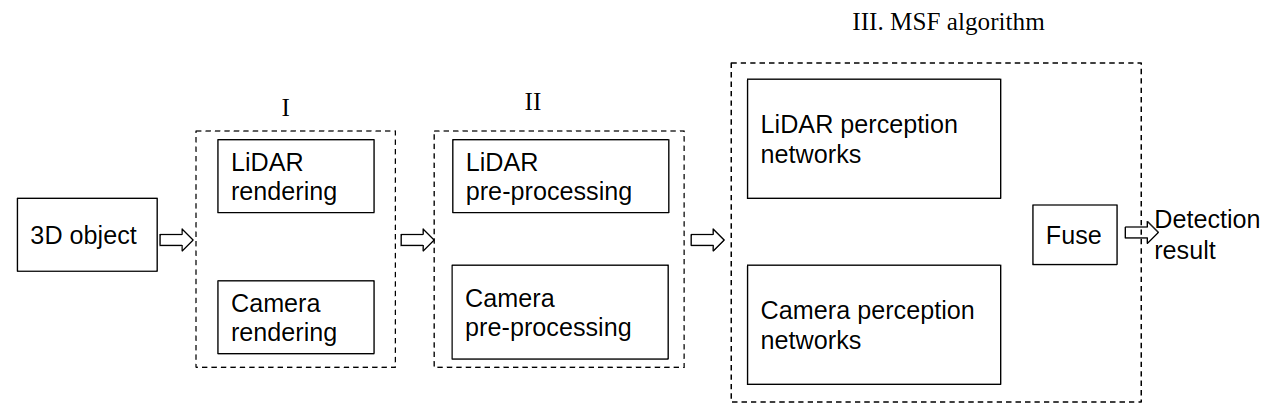
\includegraphics[width=1\linewidth]{figure/structure.png}
	\caption{Perception module in AV systems}
	\label{fig:module}
\end{figure*}
